\textbf{Problem definition}:
Consider

%
\begin{equation}\label{eq:Q2}
	\dot{x} = x^3 + \delta x - \mu x
\end{equation}
%

Determine the fixed points of the system and study the biforcations in the $(x, \mu)$ plane for non-zero values of $\delta$

\noindent\hrulefill

% -------------------------------------------------------------------
\textbf{Solution approach:} The stationary points are calculated by setting $\dot{x}$ equal to zero.

%
\begin{subequations}\label{eq:stationaryPoints}
\begin{align}
	x &= 0 \label{eq:stationary0}
	\\
	x &= \pm \sqrt{\mu - \delta} \label{eq:stationary1}
\end{align}
\end{subequations}
%

The Jacobian for Equation \eqref{eq:Q2} is calculated as

%
\begin{equation}\label{eq:jacobian}
	D_x F = 3x^2 + \delta - \mu
\end{equation}
%

where $F = x^3 + \delta x - \mu x$. The eigenvalue is written as

%
\begin{equation}\label{eq:eigenvalue}
	\lambda = 3x^2 + \delta - \mu = 2 \left( \mu - \delta \right)
\end{equation}
%

The derivative of the forcing function to the control parameter, $\mu$, is calculated as:

%
\begin{equation}
	F_\mu = -x
\end{equation}
%

For $(x, \mu) = (0, 0)$ we have the following conditions:

%
\begin{equation}
\begin{cases}
	F(0, 0) = 0 \\
	D_x F \text{ has zero eigenvalue}
\end{cases}
\end{equation}
%

Therefore, we have satisfied the necessary conditions for the bifurcations. Since $F_\mu$ is in the range of $D_x F$ at $(0,0)$, we have a pitch fork bifurcation.

Comparing Equations \eqref{eq:stationaryPoints} and \eqref{eq:eigenvalue} we can reach the following conclusions about the stability of the stationary points.

\begin{itemize}
	\item for $x = 0$, depending on the value of $\delta$ the stationary point can be come stable and unstable. For $\mu > \delta$ we have s stationary point and for the case of $\mu < \delta$ we have an unstable point.
	\item for stationary point defined by $x = \pm \sqrt{\mu - \delta}$ to exist, $\mu - \delta$ needs to be grater than zero. This means that the eigenvalue associated with point is always poisitive (Equation \eqref{eq:eigenvalue}). Hence the stationary point is always unstable.
\end{itemize}

The bifurcations plots for different values of $\delta$ are shown in Figure \ref{fig:bifurcation}.

%
\begin{figure}[h]
	\centering
	\begin{subfigure}[h]{8.0 cm}
		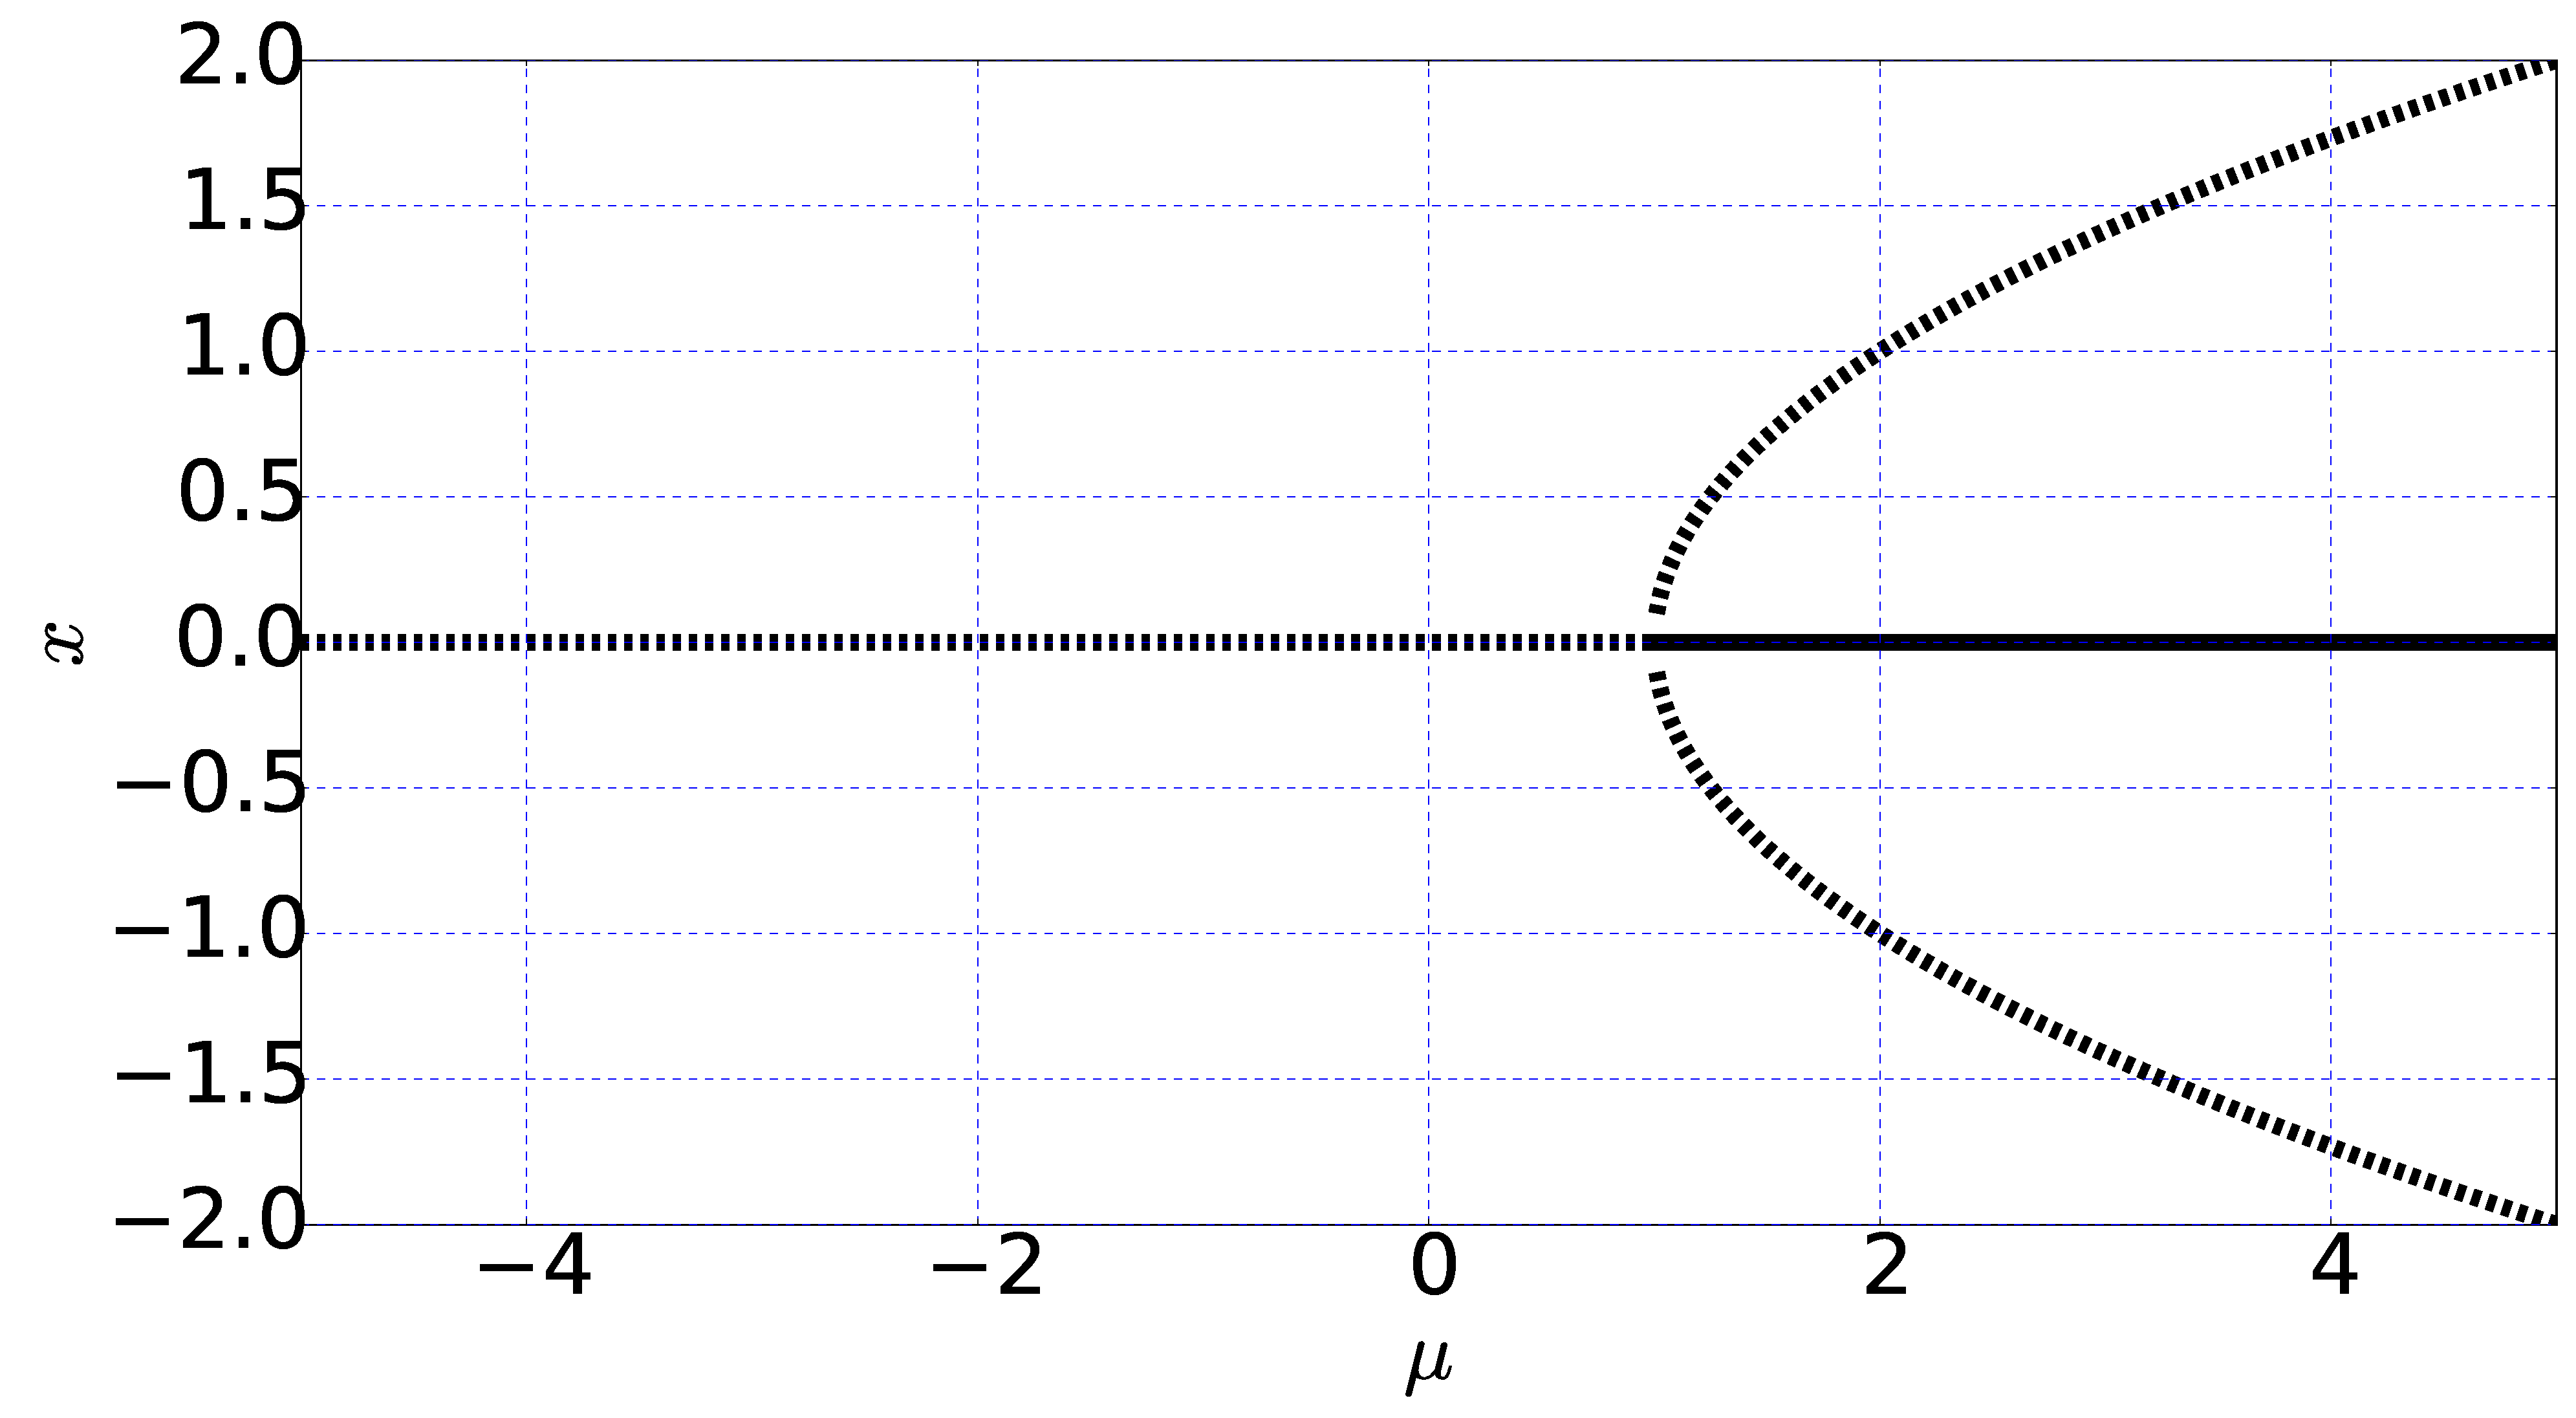
\includegraphics[width=8.0 cm]{figure/Q2/original/delta1.eps}
		\caption{$\delta = 1$}
	\end{subfigure}
	\begin{subfigure}[h]{8.0 cm}
        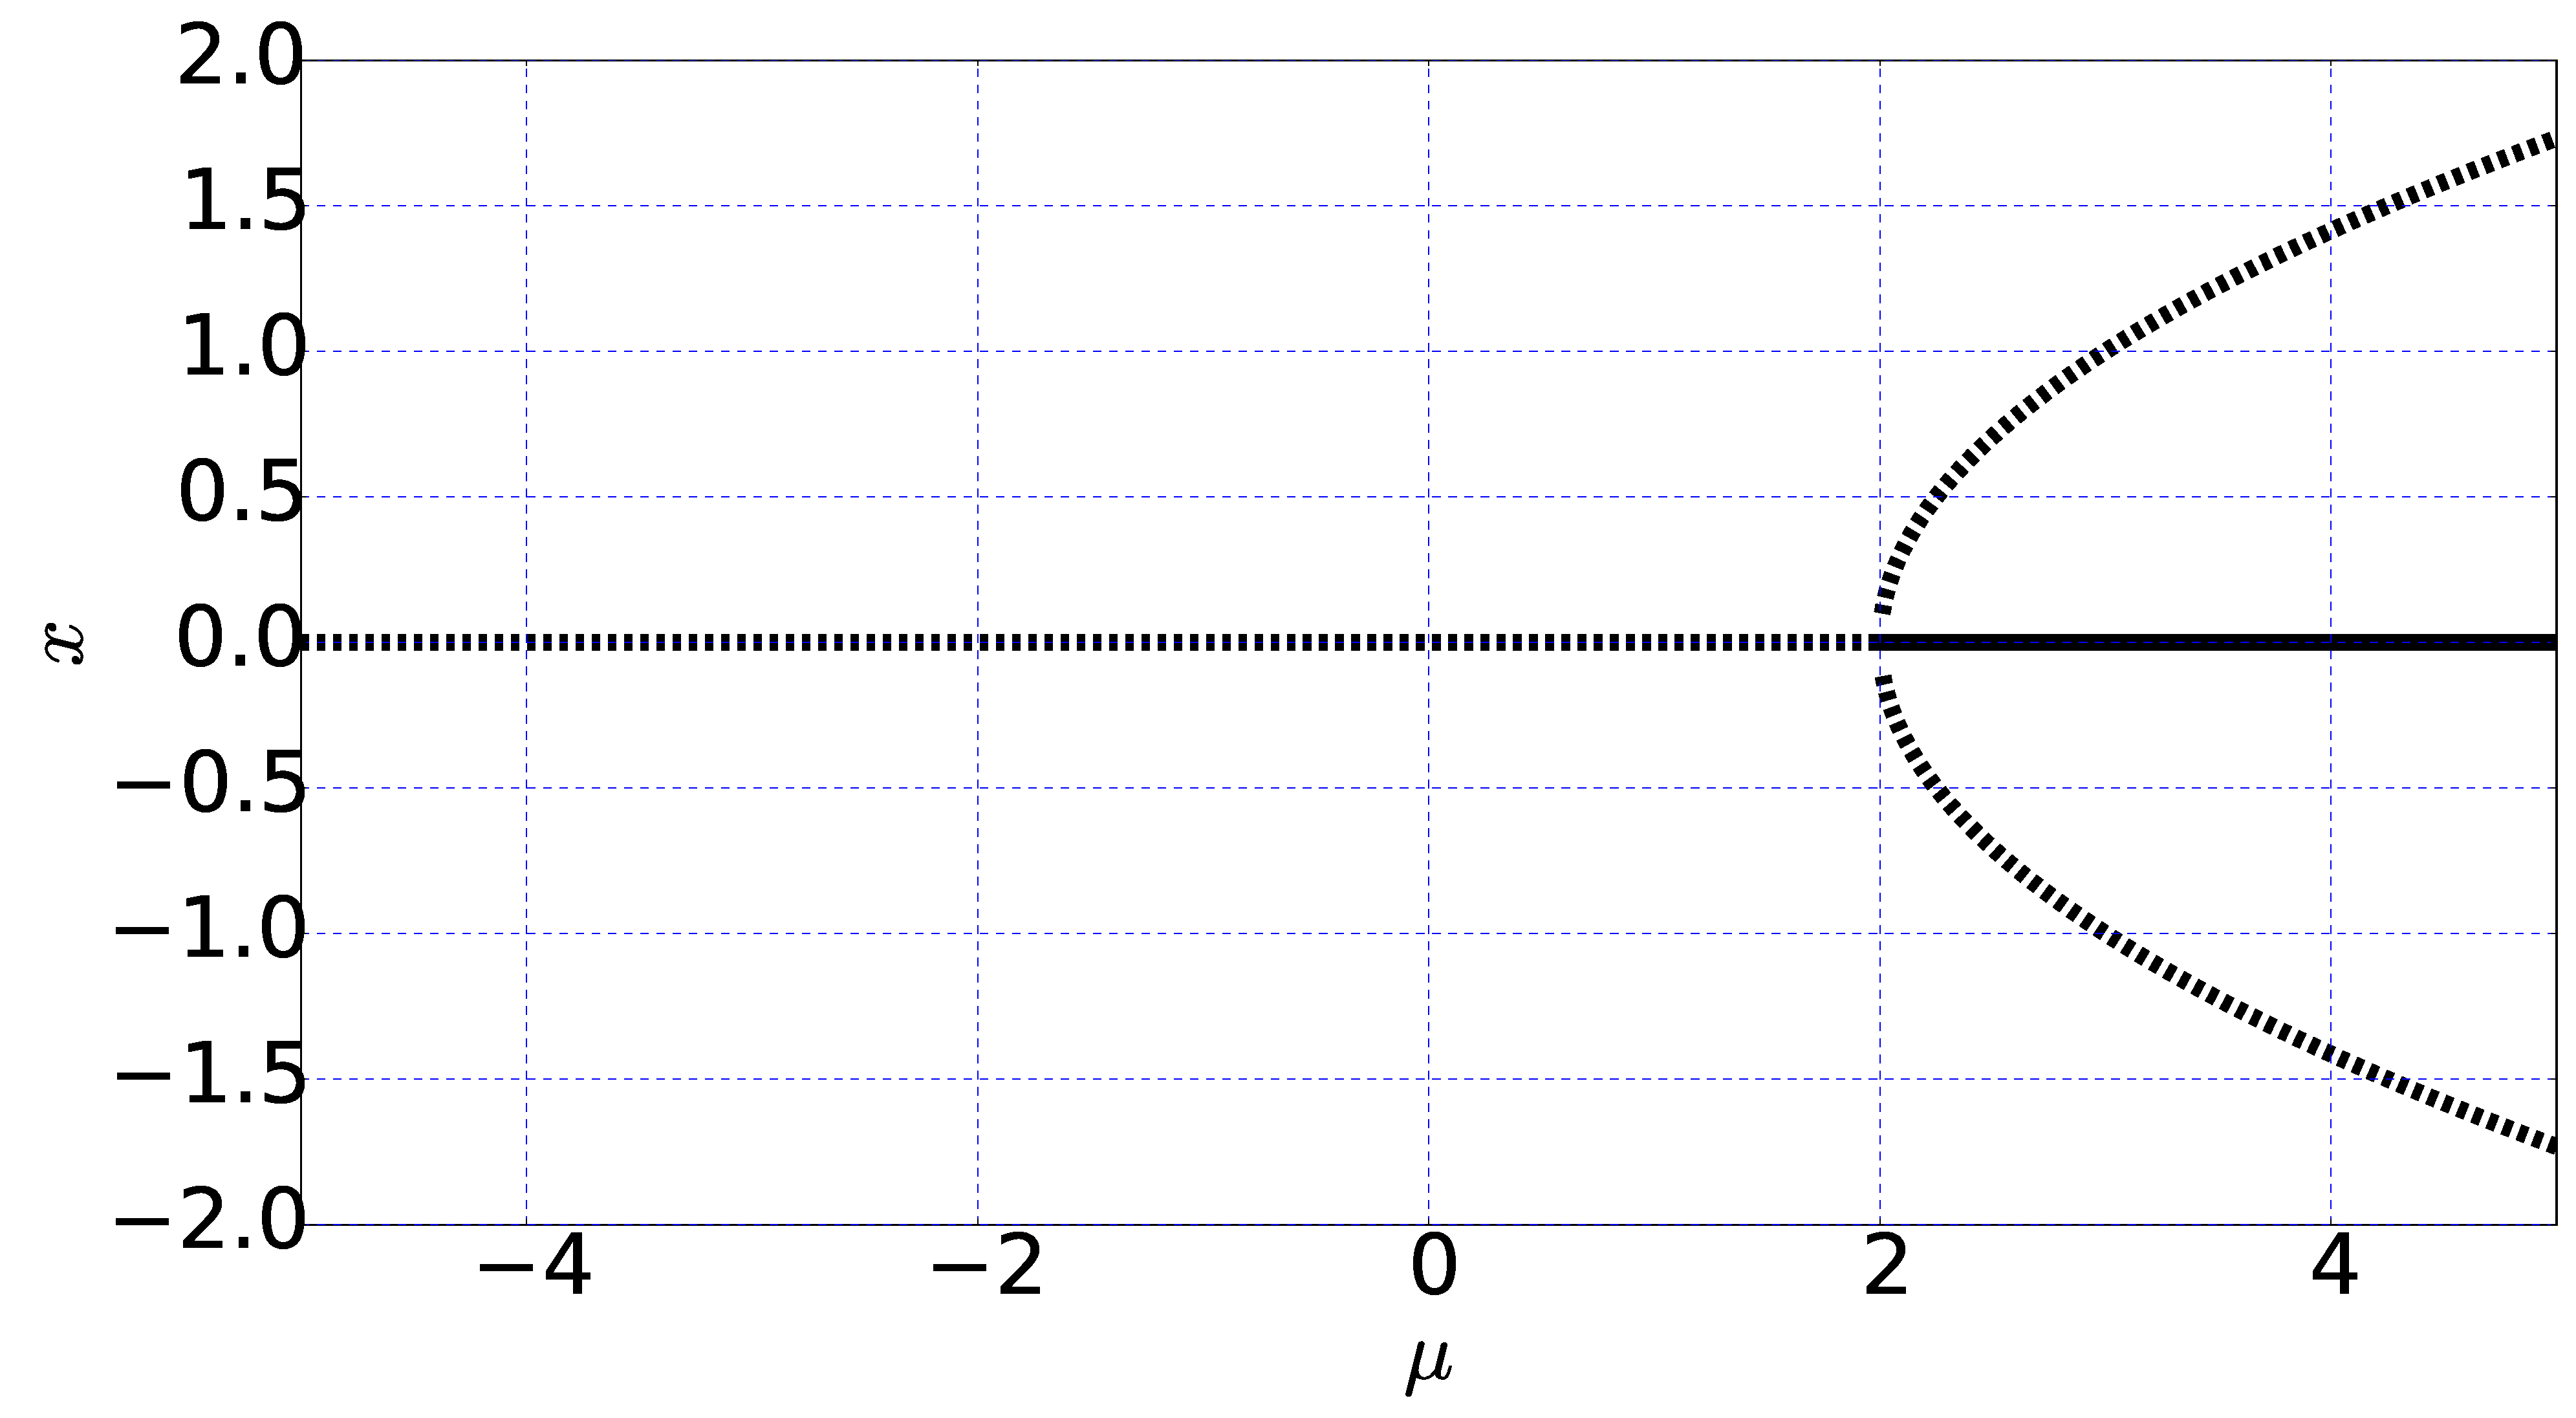
\includegraphics[width=8.0 cm]{figure/Q2/original/delta2.eps}
		\caption{$\delta = 2$}
    \end{subfigure}
    \\
    \begin{subfigure}[h]{8.0 cm}
		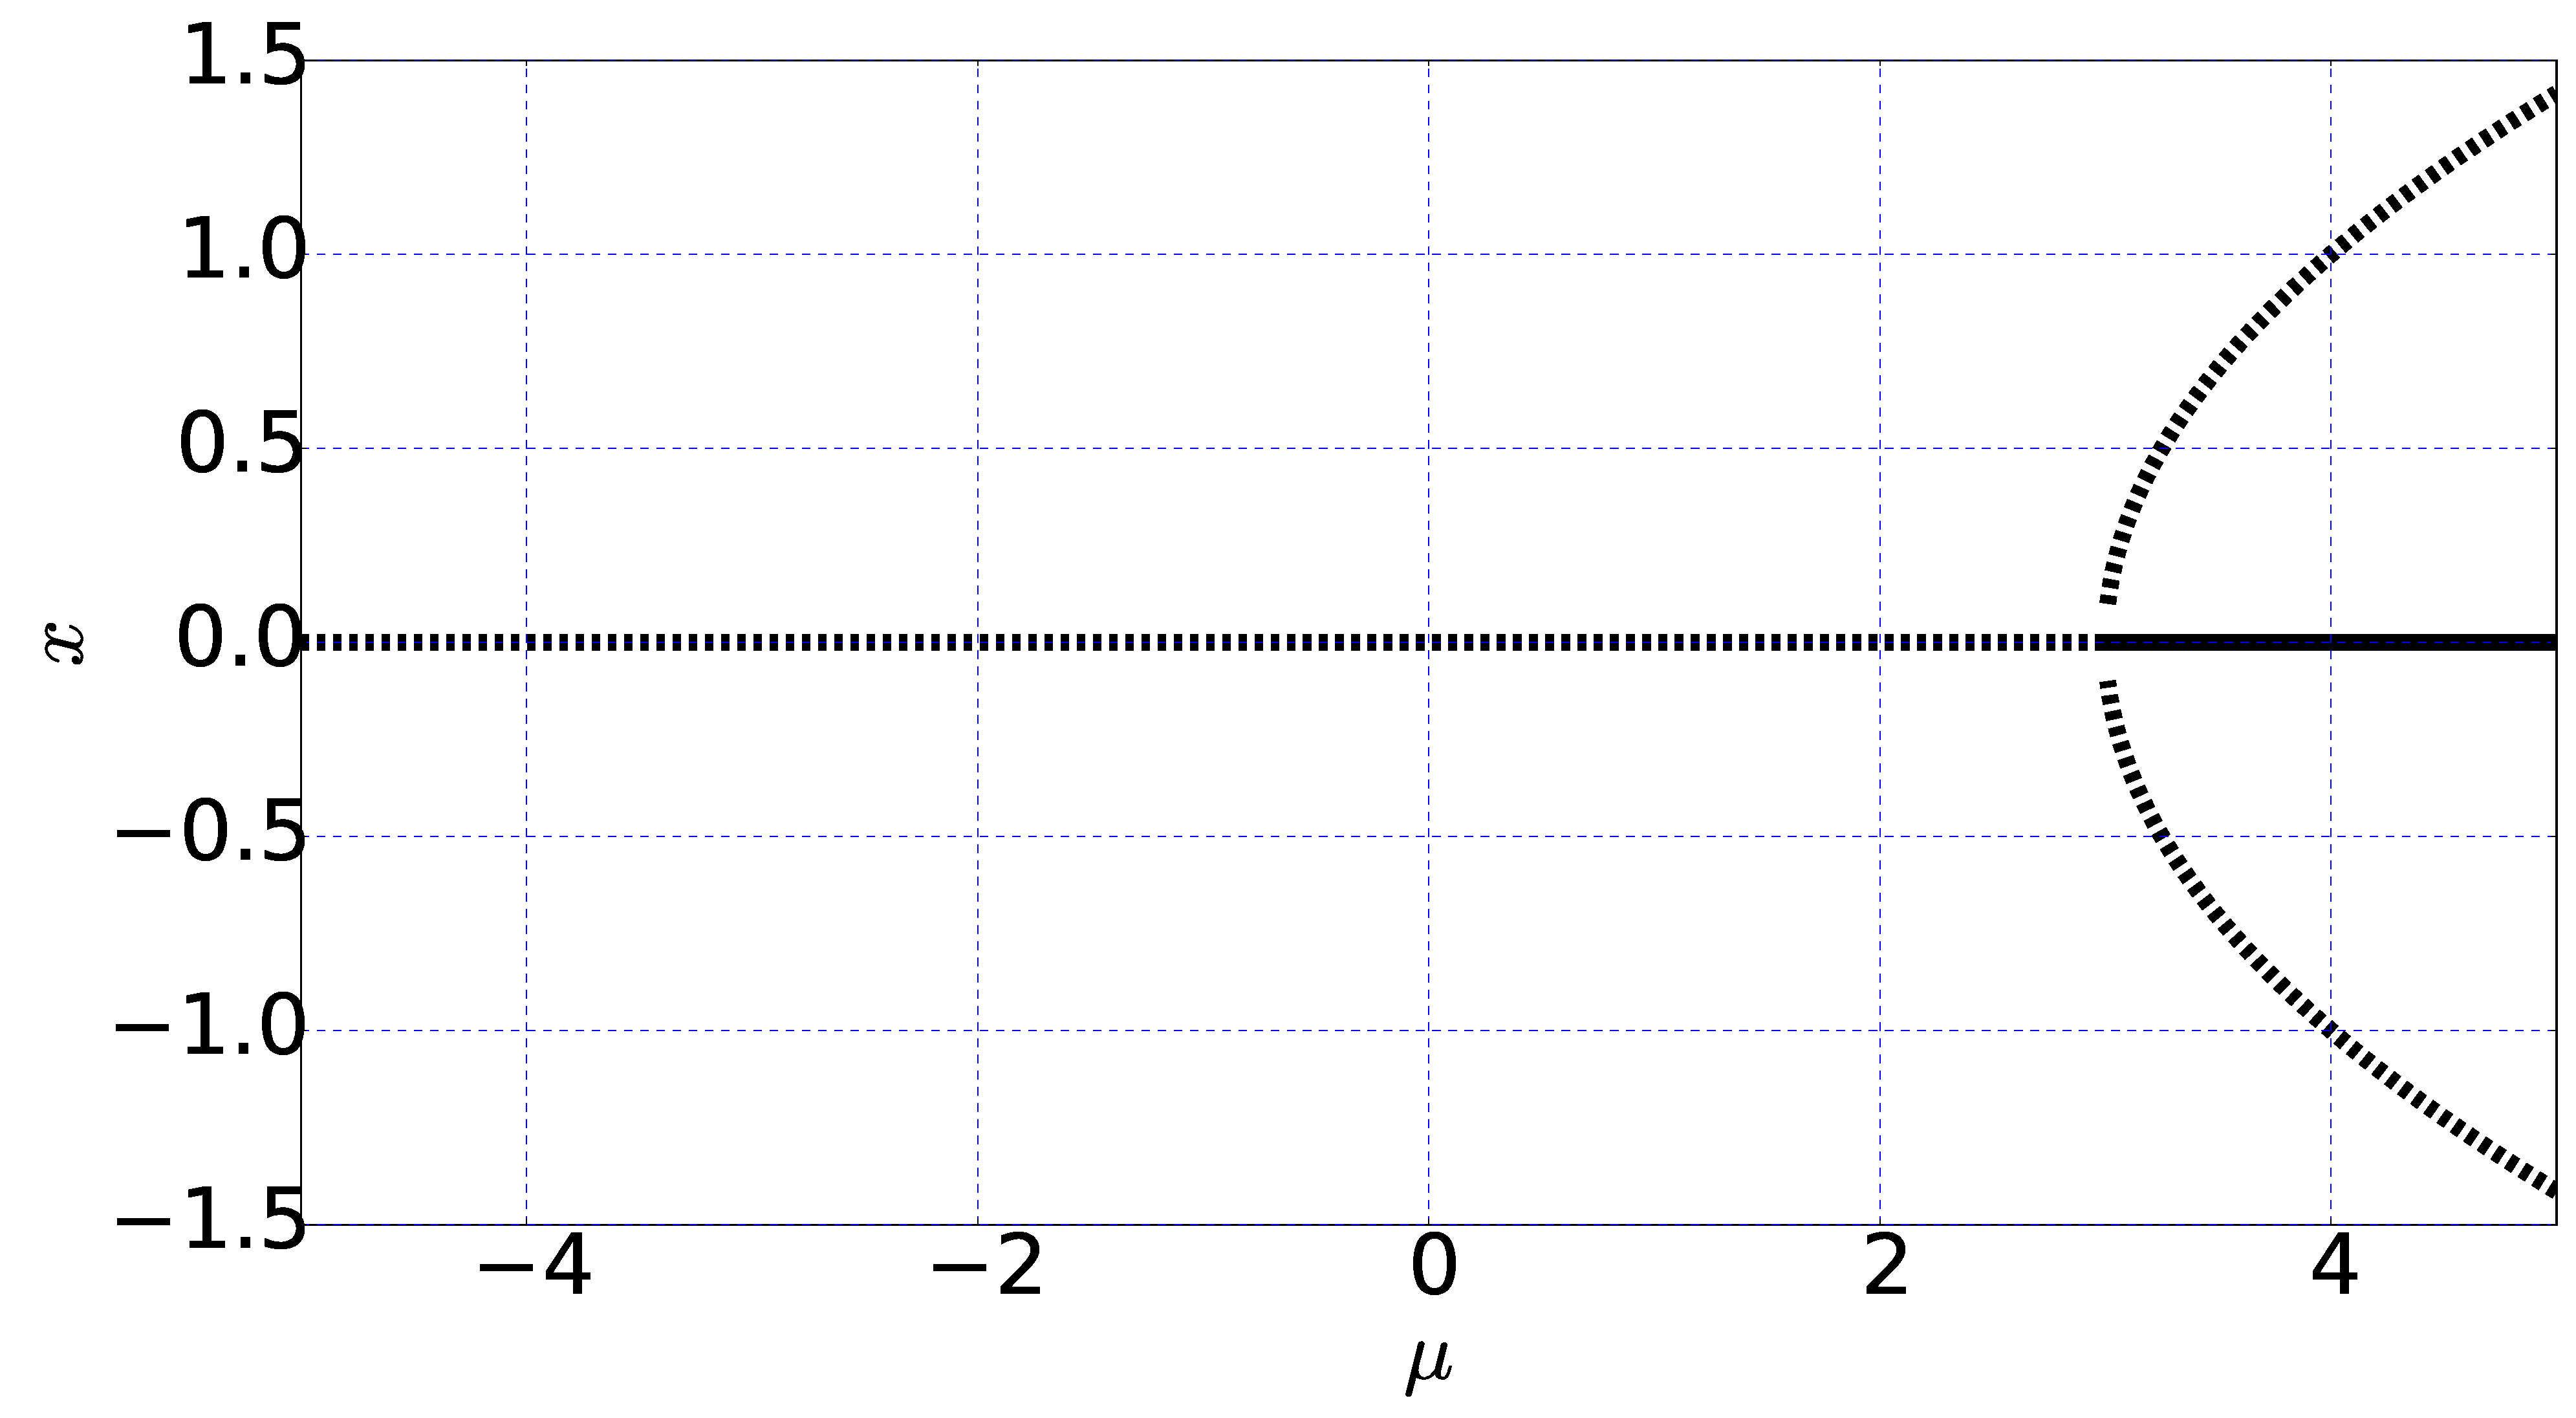
\includegraphics[width=8.0 cm]{figure/Q2/original/delta3.eps}
		\caption{$\delta = 3$}
	\end{subfigure}
	\begin{subfigure}[h]{8.0 cm}
        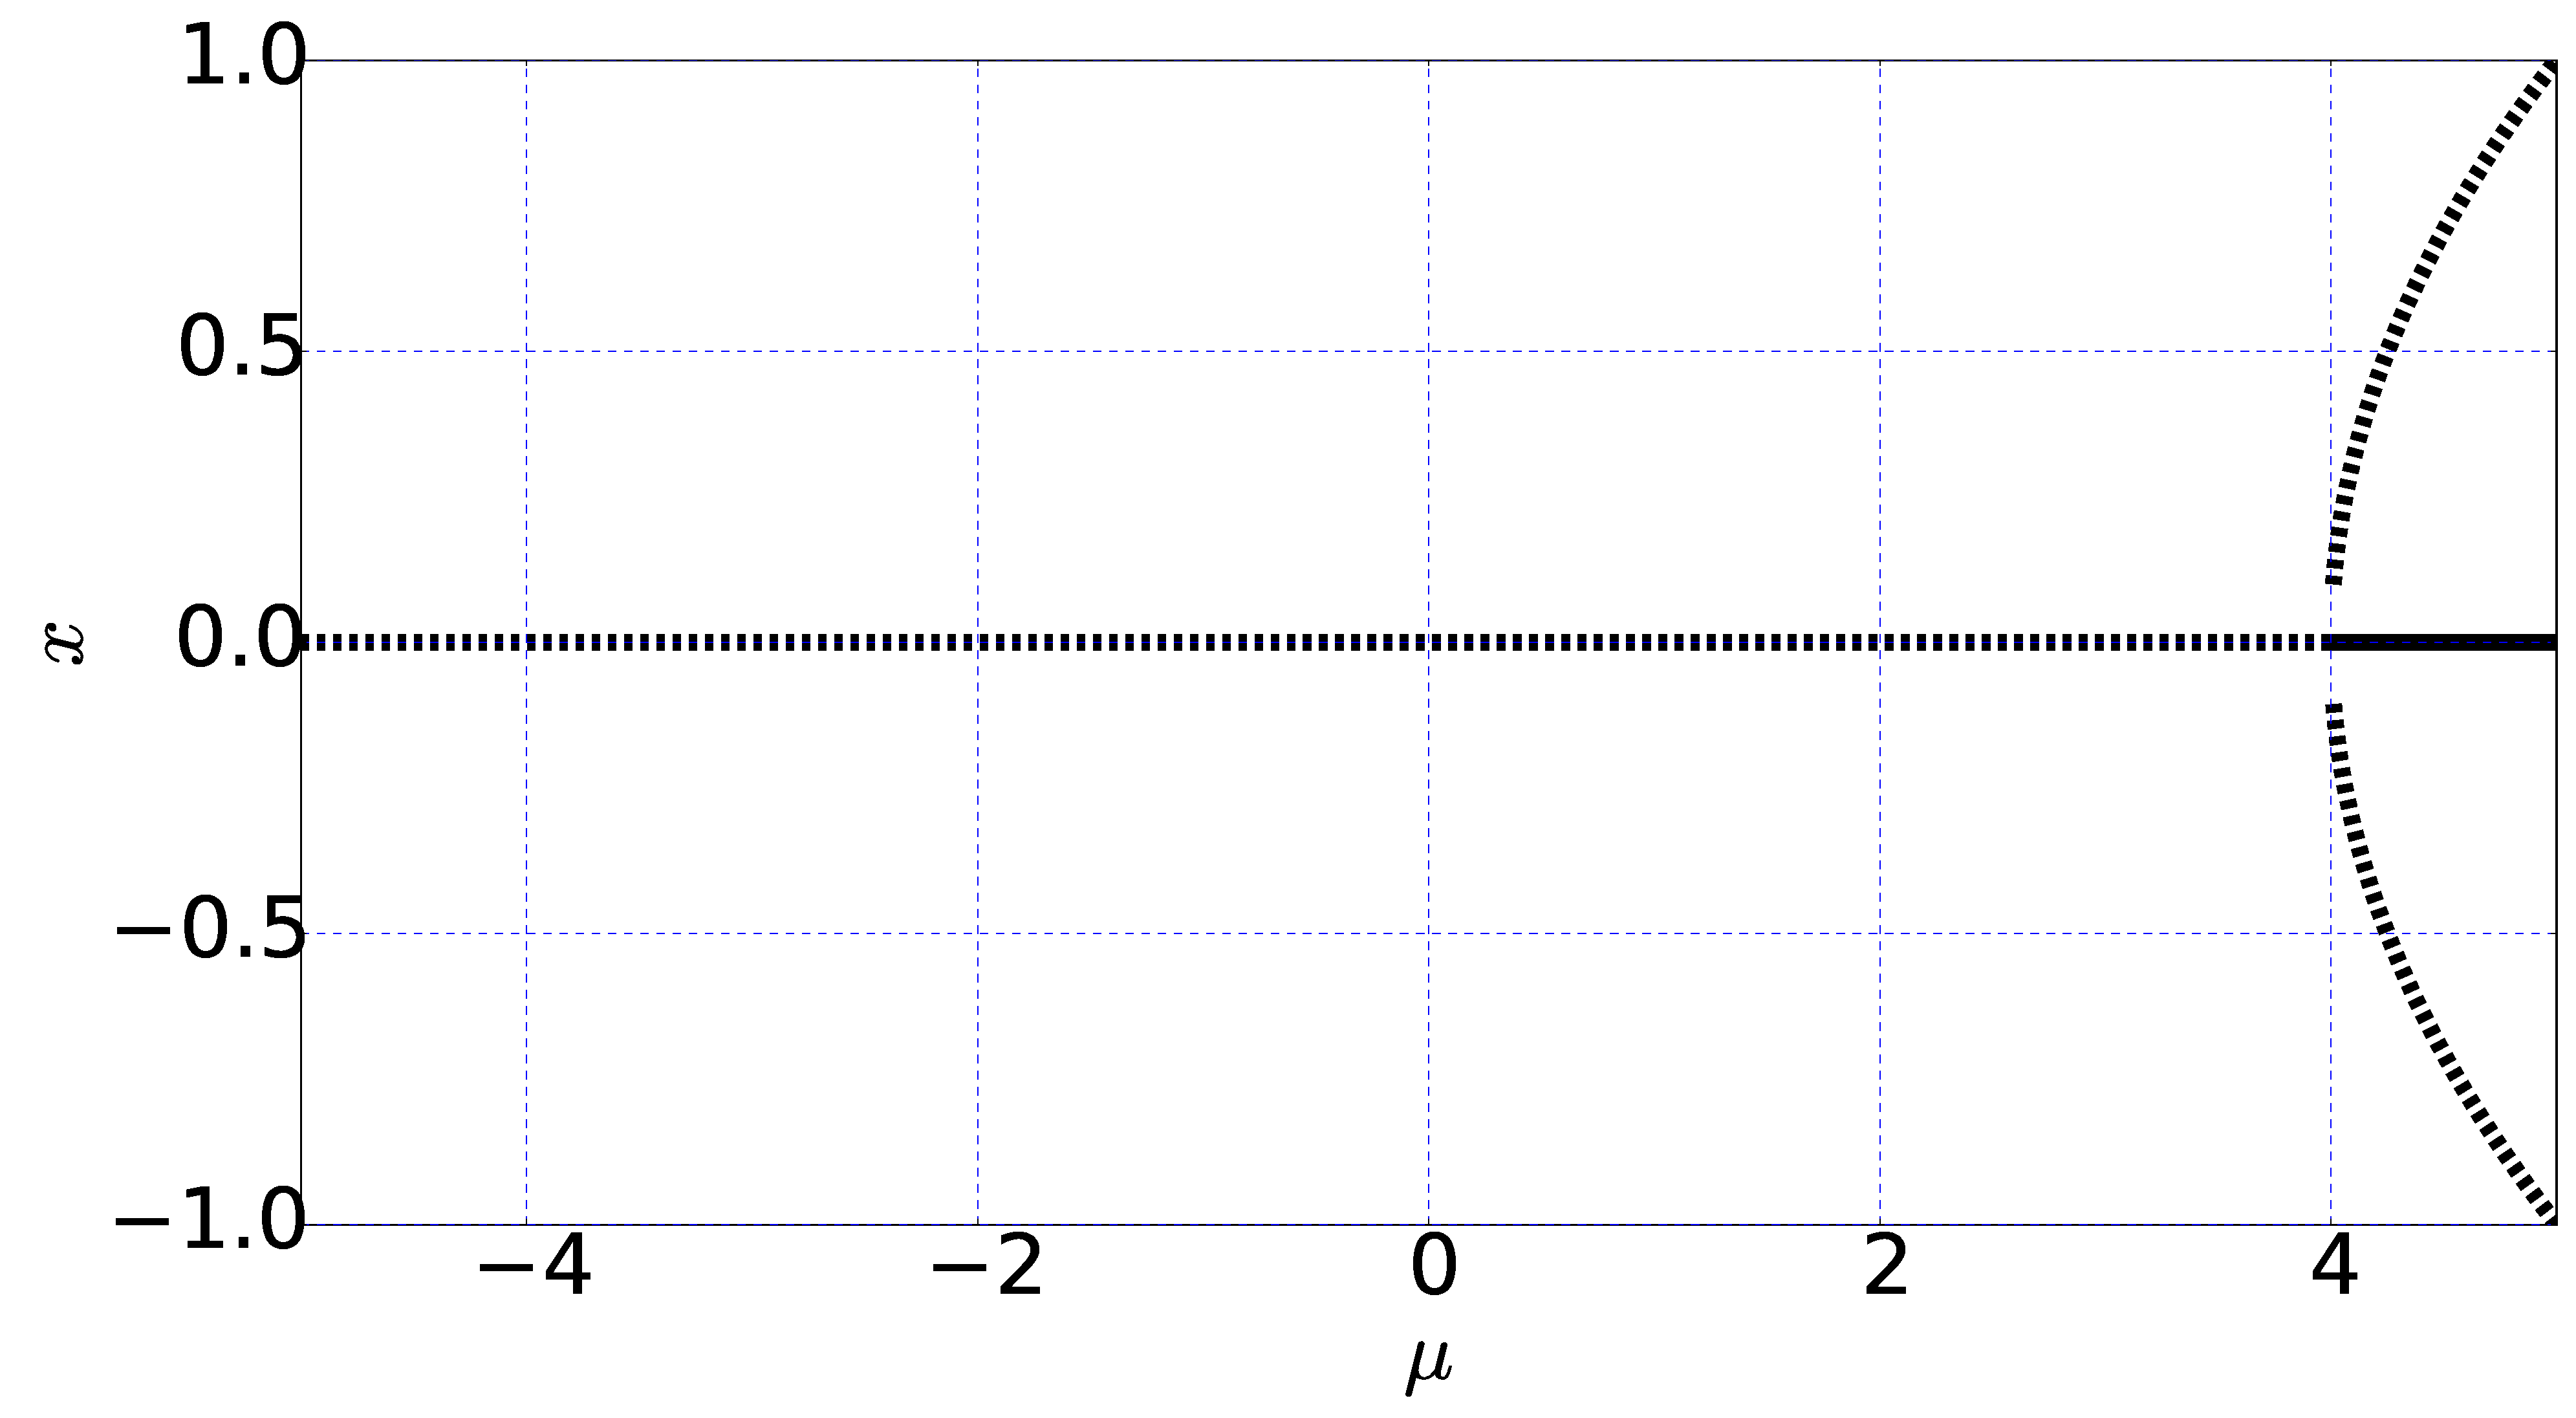
\includegraphics[width=8.0 cm]{figure/Q2/original/delta4.eps}
		\caption{$\delta = 4$}
    \end{subfigure}
    \caption{Bifurcation diagram for different positive values for $\delta$. The dashed line is the \emph{unstable branch} and the solid line is the \emph{stable branch}.}
    \label{fig:bifurcation}
\end{figure}
%